\documentclass[10pt,final,a4paper,oneside,onecolumn]{article}

%%==========================================================================
%% Packages
%%==========================================================================
\usepackage[a4paper,left=3.5cm,right=3.5cm,top=3cm,bottom=3cm]{geometry} %% change page layout; remove for IEEE paper format
\usepackage[T1]{fontenc}                        %% output font encoding for international characters (e.g., accented)
\usepackage[cmex10]{amsmath}                    %% math typesetting; consider using the [cmex10] option
\usepackage{amssymb}                            %% special (symbol) fonts for math typesetting
\usepackage{amsthm}                             %% theorem styles
\usepackage{dsfont}                             %% double stroke roman fonts: the real numbers R: $\mathds{R}$
\usepackage{mathrsfs}                           %% formal script fonts: the Laplace transform L: $\mathscr{L}$
\usepackage[pdftex]{graphicx}                   %% graphics control; use dvips for TeXify; use pdftex for PDFTeXify
\usepackage{array}                              %% array functionality (array, tabular)
\usepackage{upgreek}                            %% upright Greek letters; add the prefix 'up', e.g. \upphi
\usepackage{stfloats}                           %% improved handling of floats
\usepackage{multirow}                           %% cells spanning multiple rows in tables
%\usepackage{subfigure}                         %% subfigures and corresponding captions (for use with IEEEconf.cls)
\usepackage{subfig}                             %% subfigures (IEEEtran.cls: set caption=false)
\usepackage{fancyhdr}                           %% page headers and footers
\usepackage[official,left]{eurosym}             %% the euro symbol; command: \euro
\usepackage{appendix}                           %% appendix layout
\usepackage{xspace}                             %% add space after macro depending on context
\usepackage{verbatim}                           %% provides the comment environment
\usepackage[dutch,USenglish]{babel}             %% language support
\usepackage{wrapfig}                            %% wrapping text around figures
\usepackage{longtable}                          %% tables spanning multiple pages
\usepackage{pgfplots}                           %% support for TikZ figures (Matlab/Python)
\pgfplotsset{compat=1.14}						%% Run in backwards compatibility mode
\usepackage[breaklinks=true,hidelinks,          %% implement hyperlinks (dvips yields minor problems with breaklinks;
bookmarksnumbered=true]{hyperref}   %% IEEEtran: set bookmarks=false)
%\usepackage[hyphenbreaks]{breakurl}            %% allow line breaks in URLs (don't use with PDFTeX)
\usepackage[final]{pdfpages}                    %% Include other pdfs
\usepackage[capitalize]{cleveref}				%% Referensing to figures, equations, etc.
\usepackage{units}								%% Appropriate behavior of units
\usepackage[utf8]{inputenc}   				 	%% utf8 support (required for biblatex)
\usepackage{csquotes}							%% Quoted texts are typeset according to rules of main language
\usepackage[style=ieee,doi=false,isbn=false,url=false,date=year,minbibnames=15,maxbibnames=15,backend=biber]{biblatex}
%\renewcommand*{\bibfont}{\footnotesize}		%% Use this for papers
\setlength{\biblabelsep}{\labelsep}
\bibliography{../../bib}

%%==========================================================================
%% Define reference stuff
%%==========================================================================
\crefname{figure}{Figure}{Figures}
\crefname{equation}{}{}

%%==========================================================================
%% Define header/title stuff
%%==========================================================================
\newcommand{\progressreportnumber}{26}
\renewcommand{\author}{Erwin de Gelder}
\renewcommand{\date}{January 9, 2019}
\renewcommand{\title}{Performance assessment of automated vehicles using real-world driving scenarios}

%%==========================================================================
%% Fancy headers and footers
%%==========================================================================
\pagestyle{fancy}                                       %% set page style
\fancyhf{}                                              %% clear all header & footer fields
\fancyhead[L]{Progress report \progressreportnumber}    %% define headers (LE: left field/even pages, etc.)
\fancyhead[R]{\author, \date}                           %% similar
\fancyfoot[C]{\thepage}                                 %% define footer

\begin{document}
	
\begin{center}
	\begin{tabular}{c}
		\title \\ \\
		\textbf{\huge Progress report \progressreportnumber} \\ \\
		\author \\ 
		\date
	\end{tabular}
\end{center}

\section{Previous meeting minutes}

\begin{itemize}
	\item I received feedback from Bart on the conference paper ``real-world scenario mining for the assessment of automated vehicles.''
	\item We discussed the possibility of a journal paper describing the overall methodology. Bart suggested that it would be a good opportunity to integrate all work done as part of my PhD. I discussed with Olaf if it would be possible to get a project at TNO to work on this. TNO developed few automated driving functions (among which emerging steering assist) for European car manufactures. Therefore, Olaf an I concluded that we might want to investigate whether we can do a project with such a car manufacture in which we assess a specific automated driving function (e.g., emerging steering assist).
\end{itemize}

\section{Summary of work}

\begin{itemize}
	\item There is no news on the ontology paper, submitted to Transportation Research Part C: Emerging Technologies. I expect a decision soon, because the status is ``Ready for Decision'' for four weeks.
	\item I continued the work on the conference paper ``real-world scenario mining for the assessment of automated vehicles.'' The latest version is attached to this report. Changes are in blue font. The deadline for the conference (Intelligent Vehicle Symposium) is February 1.
\end{itemize}

\section{Future plans}

In \cref{fig:planning}, the updated planning is shown. There are a few changes compared to the planning shown in the previous progress report:
\begin{itemize}
	\item I extended the period for the ontology paper by one quarter because I am still waiting on a decision. 
	\item I extended the period for the journal paper on the overall methodology. The first step will be to define the scope of the paper and to propose a project. 
\end{itemize}

\begin{figure}[t]
	\centering
	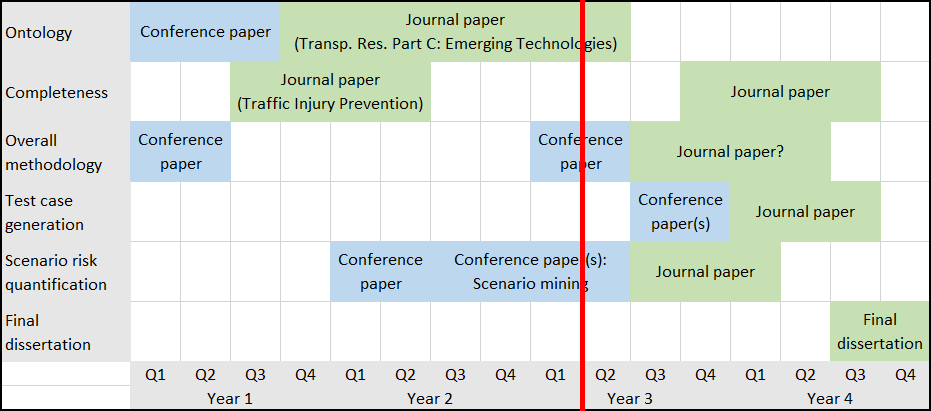
\includegraphics[width=\linewidth]{planning.png}
	\caption{Proposed planning at the time of this report. The red line indicated the time when writing this report.}
	\label{fig:planning}
\end{figure}

On the short term, I plan to work on the following:
\begin{itemize}
	\item Finish the conference paper on the scenario mining for the Intelligent Vehicle Symposium.
	\item Check internally at TNO the possibility for a project with a car manufacture to apply the work of my PhD to assess an automated driving function.
\end{itemize}

\section{Questions}

\begin{itemize}
	\item Considering the initial deadline for the conference paper for the Intelligent Vehicle Symposium, I want to finish a draft on January 19. Would it be possible to provide feedback during the following week, i.e., by January 24?
\end{itemize}


\printbibliography

\clearpage
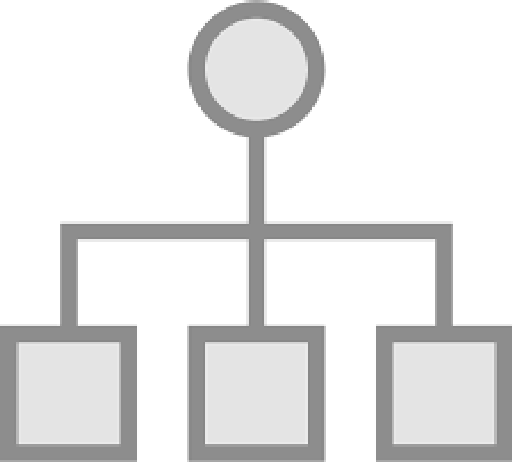
\includepdf[pages=-,pagecommand={},width=\paperwidth]{../../"20191010 Scenario Mining"/scenario_mining.pdf}

\end{document}